\section{Connessione}
Un grafo si dice \textit{connesso} se - a partire da un nodo qualsiasi - posso raggiungerne un altro qualsiasi.
Qualora non sia connesso, si definisce \textit{componente connesso} qualsiasi sezione connessa che lo compone.

\section{Visitare un grafo}
Esistono due tipi di visita:
\begin{enumerate}
    \item Visita in profondità
    \item Visita in ampiezza
\end{enumerate}

\subsection{Visita in profondità}
Rappresenta una visita ricorsiva del grafo, partendo da un nodo generico scelto arbitrariamente. \\
Si costruisce un vettore binario \textit{v} (i cui valori sono inizialmente impostati tutti a \textit{0} - con costo $O(n)$), composto da n componenti, utilizzato per tenere traccia se il nodo preso in esame è già stato visitato (e quindi il suo valore sul vettore sarà impostato ad \textit{1}) o meno. \\
\begin{center}
    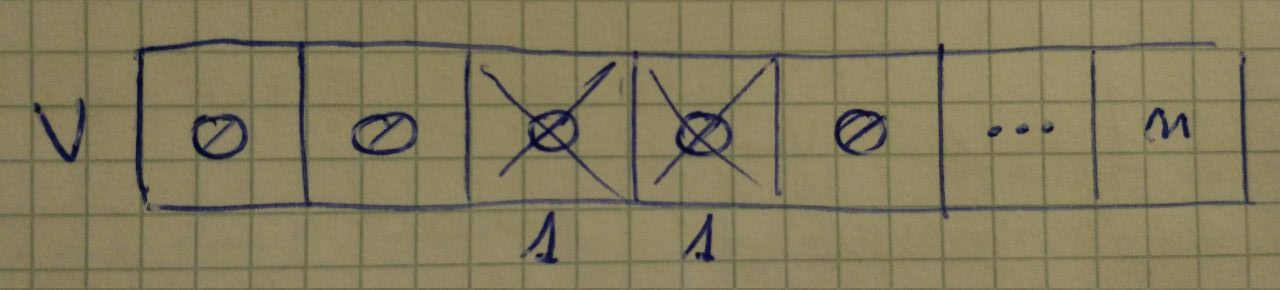
\includegraphics[width=.8\textwidth]{res/vettore-visita.jpg} \hfill
\end{center}
\newpage

L'algoritmo di \textit{visita in profondità} prende il nome di \textit{DFS}, che sta per \textit{Depth First Search}.
Inizializzato il vettore a \textit{0}, eseguo la procedura \textit{DFS(x)}:
\begin{lstlisting}
DFS(x)
    vis[x] <- 1         # imposto il valore del nodo ad 1
    for y in adj(x)     # itero sui nodi adiacenti ad x
        if vis[y]==0 then DFS(y)
\end{lstlisting}

Chiaramente, se al termine della visita \textit{v} contiene ancora alcuni \textit{0}, significa che il grafo non è connesso. \\
Genericamente la procedura \textit{DFS(x)} ha complessità di $O(n)$. Inoltre, però, questa fa un'iterazione (attraverso il ciclo \textit{for}) per ogni adiacenza col nodo, impiegando - nel caso peggiore - \textit{n} - caso in cui, quindi, il nodo abbia numero di adiacenze pari al numero totale di nodi. Di conseguenza, la procedura di visita impiega al più $O(n^2)$. \\
Se questa procedura - invece di lavorare con un vettore - lavora sulla rappresentazione a matrice, il caso peggiore che abbiamo analizzato, diventa l'unico caso possibile, per cui $\theta(n^2)$. \\
Infine, utilizzando la rappresentazione tramite liste di adiacenze, la procedura avrà complessità $O(n+m)$. \\\\
Tramite il percorso seguito dalle chiamate \textit{DFS(x)} è inoltre possibile ricavarci un albero, la cui radice è proprio la sorgente da cui si è partiti nella visita del grafo. \\
Inoltre, tramite lo stesso algoritmo - aggiungendo codice e/o funzioni - è possibile ottenere funzionalità particolari e aggiuntive, come la costruzione di un \textit{vettore dei padri}, un vettore che associa ad ogni nodo il corrispettivo padre nella rappresentazione dell'albero ottenuto tramite la visita del grafo.
\newpage

\begin{algorithm}
    \caption{Verifica di presenza di un ciclo}\label{alg:VPC}
    \begin{algorithmic}[1]
        \Function{HasCicli}{$x$}\Comment{Verifica la presenza di un ciclo}
            \State $ {vis}(x) \gets 1$ \Comment{Flag di visita}
            \For { $y \in {adj}(x)$} \Comment{Lista di adiacenza di x}
                \If ${ (a)= {true} }$
                    \Return true $(y)$ \Comment{Ricorsione per ricerca in profondità}
                \EndIf
            \EndFor
            \State \textbf{return} false\Comment{}
        \EndFunction
    \end{algorithmic}
\end{algorithm}

Secondo il professore l'algoritmo non è ottimizzato.
Prendiamo il vettore dei padri: l'unica cosa che avremmo dovuto fare per tenerlo aggiornato sarebbe stata P[n] <- e poi chiamiamo cicli(u), con questa istruzione ogni nodo saprebbe chi è il padre.

Analizziamo ora la complessità di questo algoritmo, e qui interviene il quesito secondo il quale ci chiediamo quale tipologia di implementazione del grafo dovremmo usare:
Ipotizzando di avere le liste di adiacenza: $O(n+m)$, che è la partenza del DFS(u), e vale $O(n)$. Supponiamo che il grafo sia aciclico, allora io dico che si ferma in $O(n)$, se è aciclico è un albero (in cui n = m). Se invece fosse ciclico: appena lo trovo mi fermo. Certamente creo un ciclo perché per non avere cicli possono esserci al più $n-1$, quindi non visita tutto il grafo, ma dopo al più $n-1$ si ferma: questo significa che dato un grafo, vedere se nel grafo c'è un ciclo, si può fare in $O(n)$ indipendentemente dagli archi che ho nel grafo. Ad essere precisi, se la applico non posso dire se il grafico è aciclico o meno, perché se fosse sconnesso se mi restituisce true vuol dire che c'è un ciclo che è collegato alla zona da cui comincio. Ma se risponde false, essendo sconnesso, potrebbe esserci un ciclo all'interno di una parte separata di grafo. Quindi in realtà questo algoritmo funziona solo in un grafo connesso. Per visitare anche pezzi diversi del grafo devo fare sostanzialmente più visite. \\

Se mi risponde false vado a scorrermi il vettore dei visitati, se tutto è stato visitato bene, ma se trovo un nodo che abbia valore 0 signfiica che si trova in una parte del grafo non raggiungibile, quindi vado a verificare quella parte del grafo, e se mi risponde false continuo a scorrere quello stesso vettore fino a quando il vettore è finito e tutti i nodi avranno valore 1. Non sto aumentando la complessità, perché mi costera $o(n(1))$, poi $o(n(2))$ + ... comunque sommati avrò in definitiva $O(n)$. Scritta in codice, la modifica risulta:

\begin{algorithm}
    \caption{VPC grafo non connesso}\label{alg:VPCnC}
    \begin{algorithmic}[1]
        \Function{HasCicliDisconnectedGraph}{$x$}\Comment{Verifica la presenza di un ciclo}
            \State ${vis}(x) \gets 1$ \Comment{Flag di visita}
            \For {$ i= 1 \rightarrow n$} \Comment{}
                \If {$ {vis}(i)= 0 {} $} $c \gets {ciclo}(i) $
                \EndIf
                \If {$ {}(b)= {true} $}
                    \Return true $(y)$ \Comment{}
                \EndIf
            \EndFor
            \State \textbf{return} false\Comment{}
        \EndFunction
    \end{algorithmic}
\end{algorithm}

Mentre nella visita di un grafo indiretto gli archi dell'albero risultante sono bipartiti, in quella di un grafo diretto gli archi sono \textit{quadripartiti}:
\begin{itemize}
	\item \textit{arco albero}: arco standard di un albero
	\item \textit{arco di attraversamento} o cross: arco laterale che va da destra a sinistra
	\item \textit{arco in avanti}: da antenato a discendente
	\item \textit{arco all'indietro} o back: da discendente ad antenato
\end{itemize} 
Per distinguere gli archi fwd/cross da back, si sottolinea la proprietà che i nodi che formano archi back non hanno finito la ricorsione in DFS.
Per sottolineare questa differenza, si inserisce nella funzione DFS l'istruzione che associa ad un nodo - nel vettore V - il valore 2 una volta finita la ricorsione (fuori dal for loop).\\
Per distinguere invece gli archi in avanti dai cross, occorre introdurre un nuovo vettore T che associ ogni nodo ad un valore numerico che ne indica l'ordine di visita: in questo modo sappiamo che i cross uniscono un nodo con un numero più grande (quindi visitato dopo) ad un nodo con un numero minore (viceversa per gli archi in avanti).
\paragraph{Esercizio}
Numerare ogni tipo di arco dell'albero derivato dalla visita partita dal nodo \textit{u}.\\
\begin{lstlisting}
tree = 0
back = 0
forw = 0
cros = 0
time = 0
V = [0|0|0|0|0|0|0|0|0|0|0|0|0|0|--]
T = [0|0|0|0|0|0|0|0|0|0|0|0|0|0|--]
DFS(x)
	vis[x] = 1 
	time++
	T[x] = time
	for y in adj(x)
		albero++
		if vis[y]==0
			then DFS(y)
		else
			if vis[y] == 2
				then back++
			else if t[x] < t[y]
				forw++
			else
				cross++
	vis[x] = 2
\end{lstlisting}
\newpage

\subsection{Visita in Ampiezza}
Dato un grafo, partendo da un nodo arbitrario, visito prima tutti i nodi ad esso adiacenti (nodi \textit{a distanza 1}). Poi, una volta visitati tutti, per ciascuno, visito i suoi adiacenti \textit{non visitati}. \\
L'albero formato da una visita in ampiezza è detto \textit{albero dei cammini minimi}, in quanto rappresenta il cammino più breve che intercorre tra la radice e un nodo qualsiasi del grafo. \\
L'algoritmo di \textit{visita in ampiezza} prende il nome di \textit{BFS}, che sta per \textit{Breadth First Search}.
\begin{lstlisting}
BFS(u)
	vis[u] = 1
    inizializza la coda Coda inserendo u
    while Coda != 0 do
        x = estrai dalla coda
        for y in adj(x) do
            if vis[y] = 0 then
                vis[y] = 1
                metti y in Coda
\end{lstlisting}
Analogamente, per costruire il vettore dei Padri, basta sostituire le occorrenze di \textit{vis} con il vettore \textit{Padri}. Utilizzando questa versione, costruiamo l'algoritmo per la costruzione delle distanza nodo-radice:
\begin{lstlisting}
# si inizializza il vettore Distanze a +infinito
BFS(u)
    Padri[u] = 0
    Distanza[u] = 0
    inizializza la coda Coda inserendo u
    while Coda != 0 do
        x = estrai dalla coda
        for y in adj(x) do
            if Padri[y] = 0 then
                Distanza[y] = Distanza[x] + 1
                Padri[y] = x
                metti y in Coda
\end{lstlisting}
\subsubsection{Dimostrazione correttezza algoritmo per induzione}
$\forall k \geq 0$ $\exists$ un'istante di tempo in cui:
\begin{enumerate}
    \item tutti i nodi con distanza $\leq k$ avranno il loro valore correttamente calcolato nel vettore Distanza;
    \item in quel momento, in coda ci sono solo i nodi a distanza \textit{k}.
\end{enumerate}
\paragraph{PASSO BASE.}
$k=0$ definisce il caso della radice, per il quale abbiamo in coda solo la radice.
\paragraph{PASSO INDUTTIVO}
Punto di esecuzione \textit{k} in cui ci sono tutti i nodi $\leq k$ correttamente inseriti nel vettore Distanza. Al passo successivo, aggiungerò la distanza dei nodi adiacenti con distanza $k+1$ e immediatamente dopo escluderò dalla coda quelli a distanza \textit{k}.
\subsubsection{Complessità di BFS}
Il ciclo \textit{while} ha costo pari a $O(n)$, a differenza del ciclo \textit{for} che, avendo costo al più di $O(n-1)$, seguendo un'\textit{analisi ammortizzata}, ci porterebbe a pensare che il costo totale sia di $O(n^2)$. \\
Approfondendo l'analisi, arriviamo però a considerare il fatto che, nonostante il ciclo \textit{for} sia interno a quello \textit{while}, il primo - in totale - raggiungerà al più \textit{m} interazioni. Questo ci porta a considerare il costo del ciclo \textit{while} come $O(n)$, in aggiunta al costo $O(m)$ portato da tutte le interazioni sul ciclo \textit{for}. Di conseguenza, in totale, raggiungerà una complessità di $O(n+m)$.

\section{Ponti}
I \textit{ponti} sono archi la cui rimozione sconnette il grafo. Un grafo connesso, formato da soli ponti è un albero; invece, un grafo connesso senza ponti è un ciclo. \\
Inoltre, il numero massimo di ponti in un grafo è di $n-1$, e raggiungono questo numero soltanto qualora si tratti di un albero.
\begin{center}
    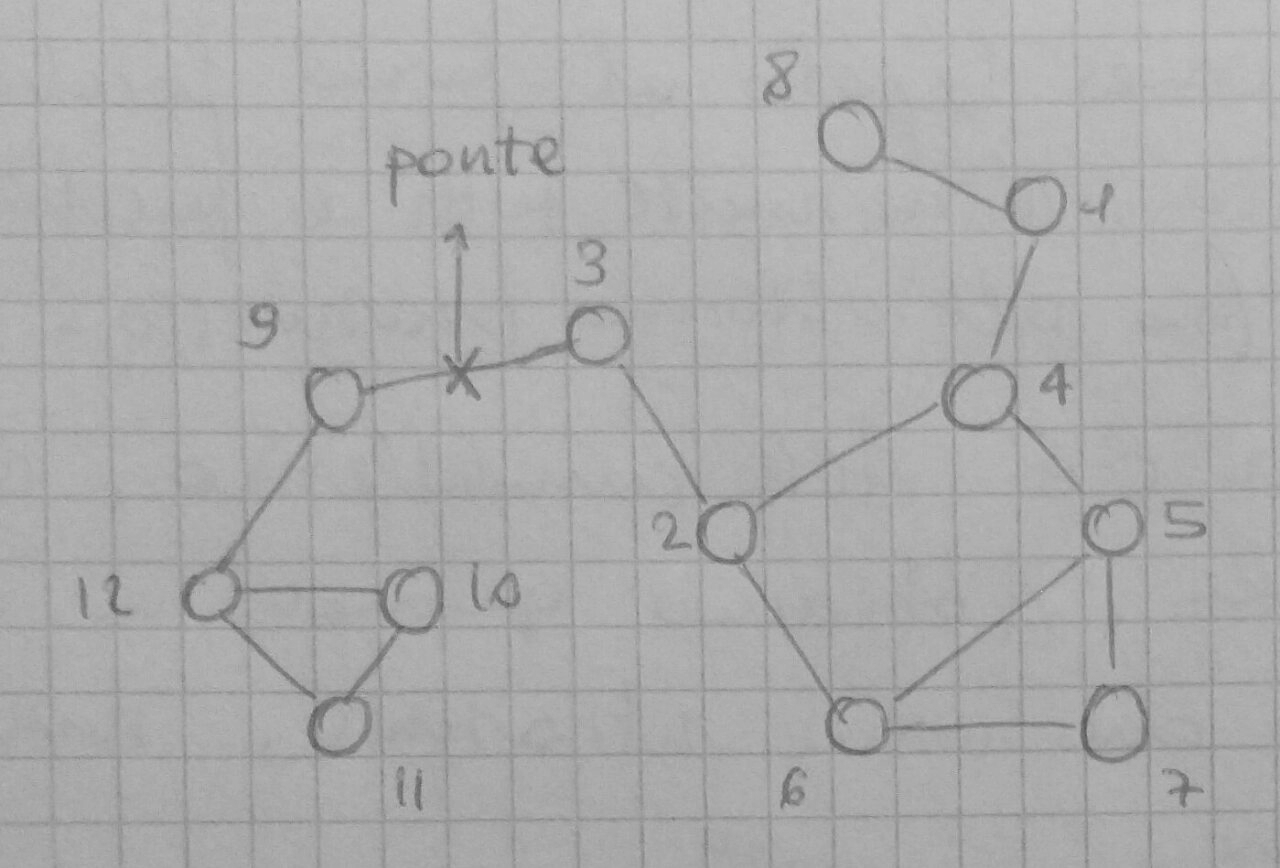
\includegraphics[width=.4\textwidth]{res/ponti-grafo.jpg} \hfill
\end{center}
Vogliamo elaborare un algoritmo che ci fornisca la lista dei ponti in un grafo.
Sappiamo che gli archi da controllare solo quelli che fanno parte dell'albero derivato dalla visita del grafo.
\begin{center}
    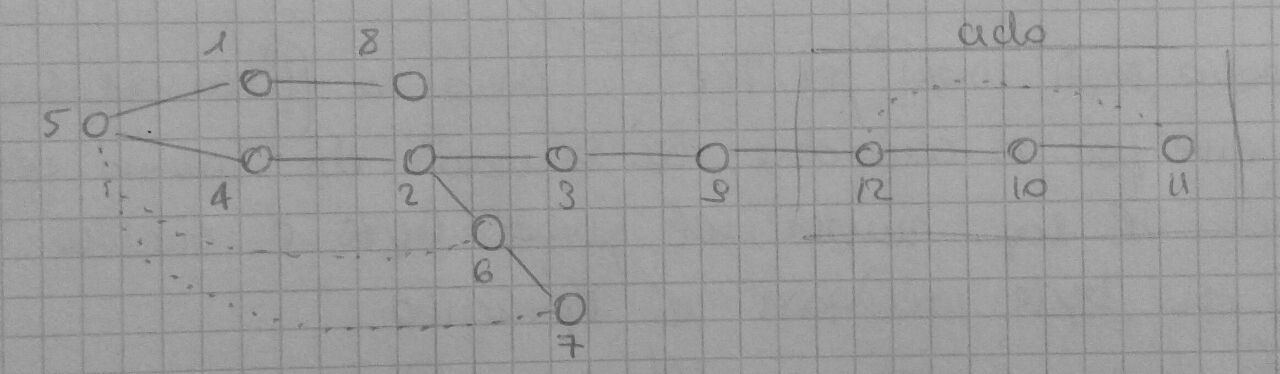
\includegraphics[width=.6\textwidth]{res/ponti-albero.jpg} \hfill
\end{center}
Tutti gli archi che non appartengono all'albero e che però erano nel grafo necessariamente non potranno essere ponti, ma saranno archi \textit{all'indietro}, \textit{in avanti} o \textit{cross}. \\
Per essere ponte, un arco deve essere arco nell'albero e non deve essere coinvolto in alcun ciclo (formato che tramite gli archi non facenti parte dell'albero). \\
Esclusi quelli, tutti i rimanenti sono ponti.
\begin{lstlisting}
# si riutilizzano i vettori Tempo, Padri, l'intero tempo
# per indicare l'ordine di visita di ciascun nodo.
DFS(u)
    tempo++
    T[u] = tempo
	vis[u] = 1 
	for y in adj(u) do
		if vis[y] = 0 then
			P[y] = u
			a = DFS(y)
			if a > T[u] then Ponti = Ponti U {y,u}
			back = min{a, back}
		else if y != P[u] then
		    back = min{T[y], back}
	return back
\end{lstlisting}
La complessità dell'algoritmo è di $O(m+n)$.

\section{Punti d'Articolazione}
I \textit{Punti d'Articolazione} sono nodi la cui rimozione sconnette il grafo. \\
In un grafo di \textit{n} nodi, questo può avere al più $n-2$ punti di articolazione. Nel caso di una catena, per esempio, . \\
Possiamo avere due tipi di alberi:
\begin{itemize}
    \item albero ad una foglia - la catena -, in cui tutti i nodi sono sicuramente punti di articolazione, esclusi il primo e l'ultimo;
    \item albero ad almeno due foglie, in cui le foglie non sono sicuramente punti articolazione.
\end{itemize}
L'algoritmo che invidivdua i punti di articolazione è molto simile a quello elaborato per individuare i ponti:
\begin{lstlisting}
# si riutilizzano i vettori Tempo, Padri, l'intero tempo
# per indicare l'ordine di visita di ciascun nodo.
DFS(u)
    tempo++
    T[u] = tempo
	vis[u] = 1 
	for y in adj(u) do
		if vis[y] = 0 then
			P[y] = u
			a = DFS(y)
			if a >= T[u] then Punti = Punti U {y}
			back = min{a, back}
		else if y != P[u] then
		    back = min{T[y], back}
    if T[u] = 1 and P[u] = 0 then
        Punti = Punti U {u}
    return back
\end{lstlisting}

\section{Sort Topologico}
Il \textit{sort topologico} rappresenta una tipologia di ordinamento lineare di grafi diretti. Nel nostro caso, desideriamo che tutti gli archi vadano solo da sinistra verso destra. \\
Non è possibile applicare questo ordinamento su tutti i grafi: infatti, l'unico caso in cui non è possibile è quello dei cicli. \\
Se è possibile applicarlo, ve ne possono essere al più $n!$ disposizioni valide diverse. \\
Un esempio banale di costruzione di un algoritmo di sorting di questo tipo è quello che seleziona per primi tutti i nodi senza archi entranti, rimuovendoli dal grafo. Se non si tratta di un ciclo, a man mano che vengono rimossi i nodi, se ne formano di nuovi senza archi entranti selezionabili, fino ad arrivare a raggiungere la situazione in cui il grafo è vuoto. \\
Prendendo come riferimento il seguente grafo:
\begin{center}
    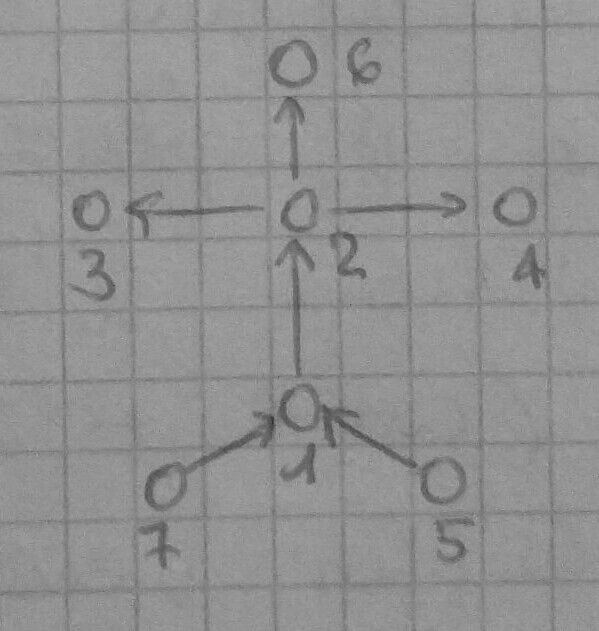
\includegraphics[width=.2\textwidth]{res/sort-topologico.jpg} \hfill
\end{center}
Un possibile output dell'algoritmo potrebbe essere la sequenza: \textit{7,5,1,2,3,6,4}.\\
Di questi, gli unici il cui ordine è fisso e non può variare senza scontrarsi con la struttura del grafo sono i due numeri \textit{1} e \textit{2}, mentre per gli altri, l'ordine è arbitrario. \\
Poiché $|\{7,5\}|=2$ e $|\{3,6,4\}|=3$, e $2!\times 3! = 2\times 1\times 3\times 2\times 1 = 12$, il numero di combinazioni possibili di sequenze che rappresentino l'ordinamento topologico del grafo è \textit{12}. \\
Avere un algoritmo che stampi \textit{tutte} i possibili ordinamenti non solo costerebbe $O((n^2)^c)$, ma il suo output sarebbe totalmente ingestibile. \\
Scriviamo quindi un algoritmo che individui \textit{uno dei} sort topologici possibili per il grafo in input:
\begin{lstlisting}
# utilizziamo una lista Sort inizialmente vuota
for i=1 to n
    if vis[i] = 0 then
        DFS[i]

DFS(u)
    vis[u] = 1
    for y in adj(u) do
        if vis[y] = 0 then DFS(y)
    aggiungi u in testa a Sort
\end{lstlisting}
Questo algoritmo costa $O(n+m)+O(n+m)$.

\section{Connessioni forti}
Si parla di \textit{grafo connesso} solo nel caso di grafi non diretti. Se il grafo è diretto occorre introdurre il concetto di \textbf{connessione forte}. \\
In un grafo, una \textbf{componente connessa} è un insieme non aumentabile di nodi raggiungibili reciprocamente a coppie. \\
Volendo definire un vettore che assegna ad ogni nodo un'etichetta diversa a seconda della sua componente, su un grafo non diretto questo vettore costa $ O(n) $ - il tempo di una visita via DFS.
Su un grafo diretto, applicare l'algoritmo sopra definito sarebbe scorretto; la direzione degli archi causa anche nei grafi diretti più semplici un livello di complessità $ O(n^2) $.